\section{Proof details}
\label{app:proofs}

\subsection{Noise-weighted projection bridge}

Let $W=\Sigma^{-1/2}P$. The constraint $P^\top\Sigma^{-1}P=I_k$ becomes $W^\top W=I_k$, and the reconstruction satisfies
\[
 \Sigma^{-1/2}\hat{s}
 =\Sigma^{-1/2}PP^\top\Sigma^{-1}x
 =WW^\top\tilde{x}.
\]
The empirical loss is therefore $N^{-1}\sum_i\|\tilde{x}_i-WW^\top\tilde{x}_i\|_2^2$. By Rayleigh--Ritz, every minimizer spans a leading rank-$k$ eigenspace of the whitened sample covariance. Mapping back yields the CW-PCA subspace. The objective depends on $W$ only through $WW^\top$, so $W$ is identified up to an orthogonal rotation.

\subsection{Whitened signal-plus-identity decomposition}

For $x=s+n$ with $s\perp n$, both zero mean, and $\mathrm{Cov}(n)=\Sigma$: independence gives $\mathrm{Cov}(x)=\mathrm{Cov}(s)+\Sigma$, and conjugating by $\Sigma^{-1/2}$,
\[
 \mathrm{Cov}(\Sigma^{-1/2}x)=\mathrm{Cov}(\Sigma^{-1/2}s)+I.
\]
Adding $I$ shifts every eigenvalue by one and changes no eigenvector, so the eigenvectors of the whitened data covariance are those of the whitened \emph{signal} covariance, in the same order. Rank-$k$ CW-PCA on noisy data therefore recovers the leading whitened signal eigenspace at the population level, which is the precise sense in which the likelihood metric supplies a self-supervised training signal.

\subsection{Kronecker-restricted bridge}

Throughout, the notation is Section~3's: a two-axis measurement $Z\in\R^{n_1\times n_2}$ with factors $U_1\in\R^{n_1\times k_1}$ and $U_2\in\R^{n_2\times k_2}$. Section~4's controlled experiment instantiates the first axis as sensor channel and the second as time, so $(n_1,n_2)=(C,T)$ and $(k_1,k_2)=(k_c,k_t)$ there and in Appendix~\ref{app:protocol}.

\begin{figure}[H]
  \centering
  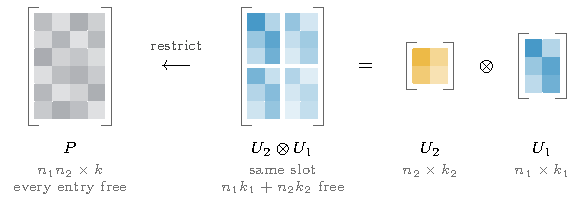
\includegraphics[width=0.78\linewidth]{figures/classes}
  \caption{What the restriction is. Both matrices are a rank-$k$ basis, $k=k_1k_2$,
  for the same vectorised two-axis measurement, so they occupy one slot; on the right the
  entries are not free, the basis being a block grid whose every block is a single
  $U_1$ motif rescaled by one entry of $U_2$. That is why the admissible family is
  the embedded product $\Gr(k_1,n_1)\times\Gr(k_2,n_2)\hookrightarrow
  \Gr(k_1k_2,n_1n_2)$ rather than the full Grassmannian, and why it costs
  $n_1k_1+n_2k_2$ parameters instead of $n_1n_2k_1k_2$. Cell counts show axis
  structure, not Section~4's sizes ($n_1=8$, $n_2=256$, $k_1=2$, $k_2=3$).}
  \label{fig:classes}
\end{figure}


For every such $Z$, the vectorization identity gives
\[
 \mathrm{vec}(U_1U_1^\top ZU_2U_2^\top)
 =(U_2U_2^\top\otimes U_1U_1^\top)\mathrm{vec}(Z).
\]
Column-stacking vectorization puts the \emph{second} axis first, which is why the admissible family is $\range(U_2)\otimes\range(U_1)$ and not the reverse. The Kronecker product is a symmetric idempotent matrix of rank $k_1k_2$, hence the orthogonal projector onto that subspace. NFPA is thus the ordinary whitened rank-$k_1k_2$ projection loss restricted to product subspaces. The restricted and unrestricted minima coincide exactly when an unrestricted minimizing projector belongs to this subset.

\subsection{Rank-one correspondence}

For $Z_i=A_i vt^\top+\epsilon_i$ with isotropic whitened noise and a unique leading signal eigendirection separated by a nonzero eigengap, the population second moment has leading vectorized direction $(t\otimes v)/(\|t\|\|v\|)$, which is feasible for rank-one NFPA. Its projection coefficient is proportional to $\langle \mathrm{vec}(Z_i),t\otimes v\rangle$, the whitened matched-filter coefficient and hence the OF amplitude up to normalization.

\begin{corollary}[Rank-one correspondence]
\label{cor:rankone}
Assume isotropic whitened noise and a unique leading population signal eigendirection separated by a nonzero eigengap. If that direction is generated by a separable template $\tilde{s}=vt^\top$, population NFPA with $k_1=k_2=1$ learns $v/\|v\|$ and $t/\|t\|$ up to signs; its scalar code is proportional to the OF amplitude of Section~2.
\end{corollary}
